% !TeX spellcheck = sk_SK-Slovak
\documentclass[a4paper]{article}
\usepackage[slovak]{babel}
\usepackage[utf8]{inputenc}
\usepackage[T1]{fontenc}
\usepackage{a4wide}
\usepackage{amsmath}
\usepackage{amsfonts}
\usepackage{amsthm,amssymb}
\usepackage{mathrsfs}
\usepackage[small,bf]{caption}
\usepackage{subcaption}
\usepackage{xcolor}
\usepackage{graphicx}
\usepackage{enumerate}
\usepackage{hyperref}
\usepackage[a4paper, total={7in, 10.2in}]{geometry}



\pagestyle{empty}
\setlength{\parindent}{0pt}

\newenvironment{modenumerate}
{\enumerate\setupmodenumerate}
{\endenumerate}

%\renewcommand{\thesubsection}{\thesection.\alph{subsection}}
\renewcommand{\thesubsection}{\alph{subsection})}


\begin{document} 
	
	\pagenumbering{arabic}
	\pagestyle{plain}
	
	\begin{center}
		\sc\large
		PHYSICAL BASED ANIMATIONS AND MATHEMATICAL MODELING HW 2 
		\\
		Matica hybnosti
	\end{center}

	Autor: Marián Kravec
	\\
	\\
	Našou úlohou je vypočítať hmotnosť, tensor zotrvačnosti a ťažisko následujúceho telesa:
	
	\centerline{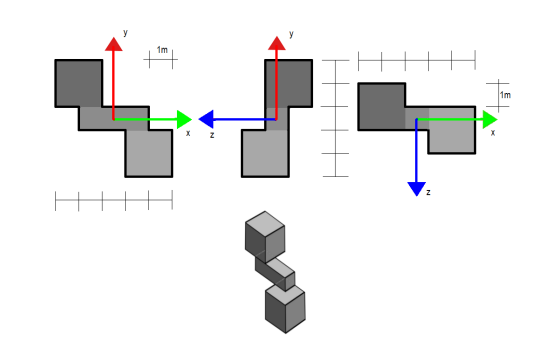
\includegraphics[width=0.7\textwidth]{podorysy}} 
	
	Prvá vec čo si môžeme všimnúť je, že aj napriek tomu, že naše teleso vyzerá pomerne komplikovane vieme ho rozdeliť na trojicu hranolov z ktorých dve hranoly sú dokonca kocky.
	\\
	\\
	To nám úlohu zjednodušuje keďže vieme, že pre hranol sa matica zotrvačnosti vypočíta následovne:
	\begin{align*}
		J_0 = \begin{bmatrix}
			\frac{m}{12}(h^2 + d^2) & 0 & 0 \\
			0 & \frac{m}{12}(w^2 + d^2) & 0 \\
			0 & 0 & \frac{m}{12}(w^2 + h^2)
		\end{bmatrix}
	\end{align*}
	Kde $(w, h, d)$ sú rozmery hranolu a $m$ je jeho hmotnosť. Avšak tento vzorec platí iba ak os otáčania prechádza ťažiskom daného hranolu. Ak je tento hranol posunutý v súradnicovej sústave o vektor $\boldsymbol{r}$ tak jeho maticu hybnosti vieme vypočítať následovne:
	\begin{align*}
		J = J_0 + m(r^TrI-rr^T)
	\end{align*}
	Poďme si teraz vypočítať rozmery jednotlivých našich rozmerov. Ak sa nemýlim v zadaní nie je ich poloha a rozmery určené presnejšie ako z pohľadu na ich vizualizáciu čiže pôdorysy. Z pôdorysov vidíme, že všetky 3 hranoly majú všetky hrany rovnobežné s niektorou zo štandardných osí čo uľahčuje určovanie ich rozmerov.
	\\
	\\
	Začnime s kockou ktorá je na pôdorysoch zobrazená ako najtmavšia, označíme si ju ako kváder $k_1$. Vidíme, že tento hranol má všetky rozmery 2 metre, ak budeme považovať meter za základnú jednotku nášho priestoru tak rozmery vieme zapísať ako $(w_1, h_1, d_1) = (2, 2, 2)$. 
	\\
	\\
	Ak sa pozrieme na kocku na opačnej strana telesa (najsvetlejšia)(označíme ako kváder $k_2$) vidíme, že jej rozmery sú totožné čiže takisto ju vieme zapísať $(w_2, h_2, d_2) = (2, 2, 2)$.
	\\
	\\
	Nakoniec nám zostal hranol v strede ktorý označíme ako kváder $k_3$. Tu si z prvého pôdorysu môžeme všimnúť, že v smere osi $x$ má náš kváder šírku $3$. Zároveň v smere osi $y$ vidíme, že má výšku $1$, hodnotu hĺbky $z$ vidíme na druhom a treťom pôdoryse a je to hodnota $1$. Takže náš kváder vieme zapísať ako $(w_3, h_3, d_3) = (3, 1, 1)$.
	\\
	\\
	Predtým, než sa pustíme do ďalších výpočtov ešte si zadefinujme hustotu tohto objektu. Keďže som sa narodil 18.9. tak v mojom prípade $x=1$ a $y=8$, čiže ak hustota je $\rho=1.xy\frac{kg}{m^3}$ tak v mojom prípade je to $\rho=1.18\frac{kg}{m^3}$.
	\\
	\newpage
	\subsection{}
	
	Ako prvé vypočítame hmotnosť celého telesa. Vieme, že celková hmotnosť telesa $m$ je súčet hmotností jeho častí. Preto ju vieme zapísať ako $m=\sum_{i=1}^{3}m_i$ kde $m_i$ je hmotnosť kvádra $k_i$.
	\\
	O hmotnosti kvádra vieme, že ju vieme vypočítať ako objem kvádra $V$ vynásobený hustotou $\rho$ ($m = V \cdot \rho$). 
	\\
	Objem kvádra vieme vypočítať ako súčin jeho rozmerov, čiže $V=w \cdot h \cdot d$
	\\
	Takže ďalším krokom bude výpočet objemu $V_i$ našich kvádrov (rozmery kvádrov sme počítali v metroch takže je to priamočiare). 
	\begin{align*}
		&V_1 = w_1 \cdot h_1 \cdot d_1 = 2 \cdot 2 \cdot 2 = 8 m^3 
		\\
		&V_2 = w_2 \cdot h_2 \cdot d_2 = 2 \cdot 2 \cdot 2 = 8 m^3 
		\\
		&V_3 = w_3 \cdot h_3 \cdot d_3 = 3 \cdot 1 \cdot 1 = 3 m^3
		\\
		&\text{Ako ďalšie vypočítame hmotnosti jednotlivých kvádrov}
		\\
		&\text{(všetky kvádre majú rovnakú hustotu $\rho$)} 
		\\
		&m_1 = V_1 \cdot \rho = 8 \cdot 1.18 = 9.44 kg
		\\
		&m_2 = V_2 \cdot \rho = 8 \cdot 1.18 = 9.44 kg
		\\
		&m_3 = V_3 \cdot \rho = 3 \cdot 1.18 = 3.54 kg
		\\
		&\text{Teraz môžeme vypočítať celkovú hmotnosť objektu}
		\\
		&m = \sum_{i=1}^{3} m_i = m_1 + m_2 + m_3 = 9.44 + 9.44 + 3.54 = 22.42 kg
	\end{align*}  
	Takže celková hmotnosť telesa je $m = 22.42 kg$.
	
	\subsection{}
	
	Ďalej chcem vypočítať tenzor zotrvačnosti $J$ pre os prechádzajúci ťažiskom telese, tento tenzor vieme vypočítať ako súčet tenzorov jednotlivých častí objektu $J = \sum_{i=1}^{3} J_i$.
	\\
	Takže teraz potrebujeme vypočítať tenzory hybnosti jednotlivých častí objektu. Nie som si istý ale mám pocit, že na to potrebujeme poznať ťažisko celého telesa, preto sa na chvíľu presunieme do časti c) kde práve túto informáciu vypočítavame.
	\\
	\\
	Ako sme  vypočítali v časti c) ťažisko nášho telesa je bod $...$, zároveň sme vypočítali, ťažiská našich jednotlivých kvádrov. Teraz potrebujeme použitím týchto informácii vypočítať vektory $r$ čiže posuny hranolov v súradnicovej sústave od ťažiska.
	
	\subsection{}
	
\end{document}
